\documentclass{article}

\usepackage{a4}
\usepackage{amsmath}
\usepackage{amsfonts}
\usepackage{amssymb}
\usepackage{float}
\usepackage[utf8]{inputenc}
\usepackage[T1]{fontenc}

\usepackage{framed}

\usepackage{graphicx}
\usepackage{caption}
\usepackage{subcaption}
\usepackage{wrapfig}

\usepackage{geometry}


\usepackage{fullpage,graphicx}
\usepackage{rotating}

\usepackage{multirow}

%\setlength{\hoffset}{-18pt}
\setlength{\oddsidemargin}{0cm}     % Marge gauche sur pages impaires
\setlength{\evensidemargin}{0cm}    % Marge gauche sur pages paires
\setlength{\marginparwidth}{54pt}   % Largeur de note dans la marge
\setlength{\textwidth}{17cm}       % Largeur de la zone de texte (17cm)
\setlength{\marginparsep}{7pt}      % Séparation de la marge
\setlength{\topmargin}{-1cm}         % Pas de marge en haut
\setlength{\headheight}{0cm}       % Haut de page
\setlength{\headsep}{10pt}          % Entre le haut de page et le texte
\setlength{\footskip}{27pt}         % Bas de page + séparation
\setlength{\textheight}{23cm}      % Hauteur de la zone de texte (25cm)

\setlength{\parskip}{1ex}
\setlength{\parindent}{1cm}

%\setlength{\topsep}{500pt}
\setlength{\abovecaptionskip}{0.1cm}
\setlength{\belowcaptionskip}{0.5cm}



\newlength{\leftbarwidth}
\setlength{\leftbarwidth}{3pt}
\newlength{\leftbarsep}
\setlength{\leftbarsep}{10pt}
\newlength{\leftbarmargin}
\setlength{\leftbarmargin}{0pt}
\newlength{\defaultparindent}
\setlength{\defaultparindent}{\parindent}


\renewenvironment{leftbar}{%
    \def\FrameCommand{\hspace{\leftbarmargin} \vrule width \leftbarwidth \relax\hspace{\leftbarsep}}%
    \MakeFramed {\advance \hsize -\width \FrameRestore }%
}{%
    \endMakeFramed
}


%\newenvironment{defx}{\noindent \\ \textbf{Definition:} \vspace{-11pt} \begin{leftbar} \vspace{4pt}}{\end{leftbar}}
%\newenvironment{propx}{\noindent \\ \textbf{Proposition:} \vspace{-11pt} \begin{framed}}{\end{framed}}

\newenvironment{defx}{
\setlength{\leftbarwidth}{3pt} 
\setlength{\leftbarmargin}{-2pt} 
\setlength{\leftbarsep}{10pt} 
\begin{leftbar}}{\end{leftbar}}
\newenvironment{propx}{\begin{framed}}{\end{framed}}

\newenvironment{demox}{\footnotesize \noindent \textit{Demo:}  \vspace{-9pt} 
\setlength{\leftbarwidth}{1pt} 
\setlength{\leftbarmargin}{5pt}
\setlength{\leftbarsep}{3pt} 
\setlength{\parindent}{7pt}

\begin{leftbar}}{\end{leftbar}
\setlength{\parindent}{\defaultparindent}
\normalsize}



\newenvironment{deft}[1]{\noindent \\ \textbf{\textsc{#1}} \vspace{-11pt} \setlength{\leftbarwidth}{3pt} 
\setlength{\leftbarmargin}{-2pt} 
\setlength{\leftbarsep}{10pt} 
\begin{leftbar} \vspace{4pt}}{\end{leftbar}}
\newenvironment{propt}[1]{\noindent \\ \textbf{\textsc{#1}} \vspace{-11pt} \begin{framed}}{ \end{framed}}


\newenvironment{algot}[1]{\noindent \\ \textbf{\textsc{#1}} \par \nobreak \vspace{1pt}\hrule\vspace{0pt} \setlength{\parindent}{0cm} \ttfamily} {\normalfont \setlength{\parindent}{\defaultparindent} \par \nobreak \vspace{4pt}\hrule\vspace{15pt}}

\newenvironment{algox}{\noindent \\  \par \nobreak \vspace{1pt}\hrule\vspace{0pt} \setlength{\parindent}{0cm} \ttfamily} {\normalfont \setlength{\parindent}{\defaultparindent} \par \nobreak \vspace{4pt}\hrule\vspace{15pt}}

%\newenvironment{algot}[1]{\noindent \\ \textbf{\textsc{#1}} \par \nobreak \vspace{1pt}\hrule\vspace{0pt} \setlength{\parindent}{0cm} \ttfamily \begin{tabbing} ~~~~\=~~~~\=~~~~\=~~~~\=~~~~\=~~~~\=~~~~} {\end{tabbing} \normalfont \setlength{\parindent}{\defaultparindent} \par \nobreak \vspace{4pt}\hrule \\}

\newcommand{\comment}[1]{\hfill// #1}

\newcommand{\bbB}{\mathbb{B}}
\newcommand{\bbN}{\mathbb{N}}
\newcommand{\bbZ}{\mathbb{Z}}
\newcommand{\bbR}{\mathbb{R}}

\newcommand{\tb}{.~~~~}

%\newcommand{\exsubpart}[1]{\subsection*{#1)}\\ }
\newcommand{\exsubpart}[1]{\subsection*{#1)} \vspace{-51pt} ~\\}

\newcommand{\info}[1]{\small{\textit{(#1)}}}




\begin{document}

\noindent {\fontsize{20}{20}\selectfont \noindent \textbf{Laboratoire d'électronique~:}}

\noindent {\fontsize{30}{30}\selectfont \noindent \textbf{Convertisseurs A/N et N/A}}

\vspace{5pt}\hrule\vspace{2pt}

\noindent {\Large \textbf{\textsc{Masur} Jonathan}\hfill \textbf{\textsc{Gosselin} Paul}}

\vspace{20pt}


On s'intéresse ici à l'étude de convertisseurs analogique/numérique (aussi appelé ``CAN'' ou ``ADC'' --- pour ``\textit{Analog-to-Digital Converter}'') et numérique/analogique (aussi appelé ``CNA'' ou ``DAC'' --- pour ``\textit{Digital-to-Analog Converter}'').

\section{Le convertisseur analogique/numérique ADC0820}
\label{sec:ADC0820}

\subsection{Prévisions théoriques}

\exsubpart{1}

Les convertisseurs analogique/numérique flash sont fréquemment utilisés, parce qu'ils permettent des fréquences de fonctionnement élevées. Toutefois, il se caractérisent en revanche généralement par des coûts énergétique et spatial élevés.

Le principe d'un CAN flash $n$ bits est le suivant.
Supposons que les valeurs analogiques à convertir soient comprises entre deux tensions de référence $V_{min}$ et $V_{max}$, fournies au convertisseur. 
$2^n$ résistances permettent de diviser $[V_{min},V_{max}]$ en $2^n$ sous-ensembles $([V_{i-1},V_i])_{i\in[1..2^n]}$ ($V_0=V_{min}$, $V_{2^n}=V_max$, $\forall i\in[1..2^n], V_i> V_{i-1}$), en fournissant les $2^n-1$ tensions de transition $V_i$.
$2^n-1$ comparateurs permettent alors de situer la tension d'entrée $V_{in}$ du condensateur par rapport à ces $2^n-1$ tensions de transition $V_i$.
Un encodeur $n$ bits --- entièrement numérique donc --- permet alors de convertir les sorties de ces comparateurs ($2^n-1$ bits) en l'entier $i$ correspondant sur $n$ bits~: $V_{in}\in[V_{i-1},V_i]$.

\begin{figure}[h]
  \centering
  \begin{subfigure}[b]{0.4\textwidth}
    \centering
    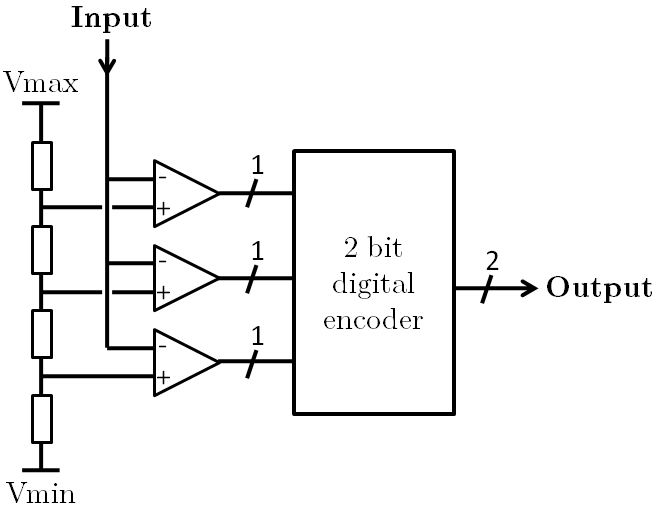
\includegraphics[width=\textwidth]{2bitFlash}
    \caption{CAN flash 2 bits}
    \label{fig:flash}
  \end{subfigure}
  ~~~~~~~~
  \begin{subfigure}[b]{0.4\textwidth}
    \centering
    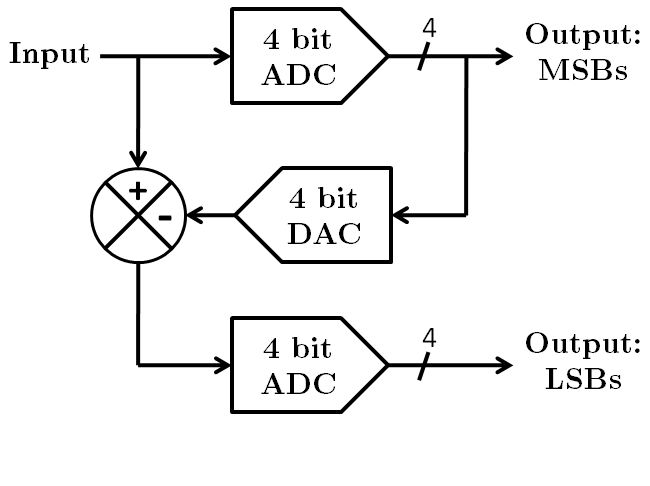
\includegraphics[width=\textwidth]{8bitSemiFlash}
    \caption{CAN semi-flash 8 bits}
    \label{fig:semiflash}
  \end{subfigure}
  \caption{Principes de base des CAN flash et semi-flash}
\end{figure}

L'un des principaux inconvéniants d'une telle structure réside dans le nombre de composants utilisés~: 

Pour limiter le nombre de comparateurs les convertisseurs semi-flashs utilisent plusieurs convertisseurs flashs. Typiquement, un convertisseur semi-flash 8 bits utilisera tout d'abord un convertisseur flash 4 bits afin d'encoder les 4 bits de poids fort (ou ``MSBs''~: ``\textit{Most Significant Bits}''). La tension $V_{MSB}$ correspondante au résultat fourni par ce convertisseur est alors soustraite à la tension d'entrée $V_{in}$, puis $V_{in}-V_{MSB}$ est traitée par un nouveau convertisseur flash 4 bits afin d'obtenir les 4 bits de poids faible (ou ``LSBs''~: ``\textit{Less Significant Bits}'').

La réactivité du convertisseur est ainsi diminuée par rapport à un convertisseur flash d(un facteur légèrement supérieur à 2, mais le nombre de composants nécessaires passe de $O(2^n)$ à $O(2^{n/2})$.
%TODO: sample & hold?

Le convertisseur analogique/numérique utilisé dans ce travail est un CAN semi-flash 8 bits~: l'ADC0820.


\exsubpart{2}

Idéalement, l'intervalle $[V_{min},V_{max}]$ est subdivisé en intervalles de même largeur. Les tensions de transitions d'une valeur à l'autre en sortie du CAN sont donc données par la formule~:
\begin{equation*}
\forall i\in[1..2^n-1], V_i = V_{min}+i\cdot\frac{V_{max}-V_{min}}{2^n}
\end{equation*}
(On rappelle que $V_i$ est la tension de transition des eniers $i-1$ à $i$ en sortie du CAN.)

Dans le cadre de notre expérience~: $V_{min}=0$ et $V_{max}=V_{ref}=\mathrm{5 V}$. Ainsi~:
\begin{equation*}
\forall i\in[1..2^8-1], V_i = i\cdot\frac{V_{ref}}{2^8} = i\cdot \mathrm{19,531 mV}
\end{equation*}

Les valeurs de $V_i$ correspondantes ont été rajouté au tableau~\ref{tab:ADC0820} des résultats expérimentaux.


\subsection{Mesures}

\exsubpart{1}

La tension d'alimentation utilisée pour le convertisseur, servant aussi de tension de référence $V_{ref}$, est fournie par une alimentation stabilisée. Elle est précisément de~: ${V_{ref}=\mathrm{4.997 V}}$.


\exsubpart{2,3}

À l'aide d'un potentiomètre 10 tours, on fait varier la tension d'entrée $V_{in}$ du convertisseur analogique / numérique étudier afin de mesurer les tensions de transition $V_i$, pour lesquelles l'entier en sortie du convertisseur --- entier représenté en binaire par des DEL --- passe de $i-1$ à $i$.

\begin{table}[h]
\caption{Résultats obtenus lors de l'étude du convertisseur ADC0820}
\label{tab:ADC0820}
\centering
\begin{tabular}{|c|c|c|c|c|c|c|c|}
\hline
$i$             & 0 & 1 & 2 & 3 & 4 & 5 & 6\\
\hline
$V_i$ théorique (V) & 0,02 & 0,039 & 0,059 & 0,078 & 0,098 & 0,117 & 0,137 \\
\hline
$V_i$ mesuré (V)    & 0,012 & 0,033 & 0,05 & 0,073 & 0,089 & 0,111 & 0.128 \\
\hline
$(V_i-V_{i-1})$ mesuré (V) & --- & 0,021 & 0,017 & 0,023 & 0,016 & 0,022 & 0,017\\
\hline
\end{tabular}

\vspace{10pt}

\begin{tabular}{|c|c|c|c|c|c|c|c|}
\hline
$i$             & 121 & 122 & 123 & 124 & 125 & 126 & 127 \\
\hline
$V_i$ théorique (V) & 2,381 & 2,401 & 2,42 & 2,44 & 2,459 & 2,479 & 2,499 \\
\hline
$V_i$ mesuré (V)    & 2,371 & 2,386 & 2,411 & 2,427 & 2,449 & 2,466 & 2,486 \\
\hline
$(V_i-V_{i-1})$ mesuré (V) & --- & 0,015 & 0,025 & 0,016 & 0,022 & 0,017 & 0,02 \\
\hline
\end{tabular}

\begin{tabular}{|c|c|c|c|c|c|c|c|}
\hline
$i$             & 128 & 129 & 130 & 131 & 132 & 133 & 134 \\
\hline
$V_i$ théorique (V) & 2,518 & 2,538 & 2,557 & 2,577 & 2,596 & 2,616 & 2,635 \\
\hline
$V_i$ mesuré (V)    & 2,507 & 2,529 & 2,544 & 2,567 & 2,583 & 2,606 & 2,622 \\
\hline
$(V_i-V_{i-1})$ mesuré (V) & 0,021 & 0,022 & 0,015 & 0,023 & 0,016 & 0,023 & 0,016 \\
\hline
\end{tabular}

\vspace{10pt}

\begin{tabular}{|c|c|c|c|c|c|}
\hline
$i$             & 250 & 251 & 252 & 253 & 254 \\
\hline
$V_i$ théorique (V) & 4,899 & 4,919 & 4,938 & 4,958 & 4,977 \\
\hline
$V_i$ mesuré (V)    & 4,883 & 4,907 & 4,922 & 4,944 & 4,961 \\
\hline
$(V_i-V_{i-1})$ mesuré (V) & --- & 0,024 & 0,015 & 0,022 & 0,017 \\
\hline
\end{tabular}
\end{table}

Ces résultats, comparés aux résultats théoriques donnés par ${V_i = i\cdot\frac{V_{ref}}{2^8}}$ et ${V_{ref}=4,997\mathrm{V}}$ sont représentés Fig.~\ref{fig:ADCres1}.

\begin{figure}
  \centering
  \begin{subfigure}[b]{\textwidth}
    \centering
    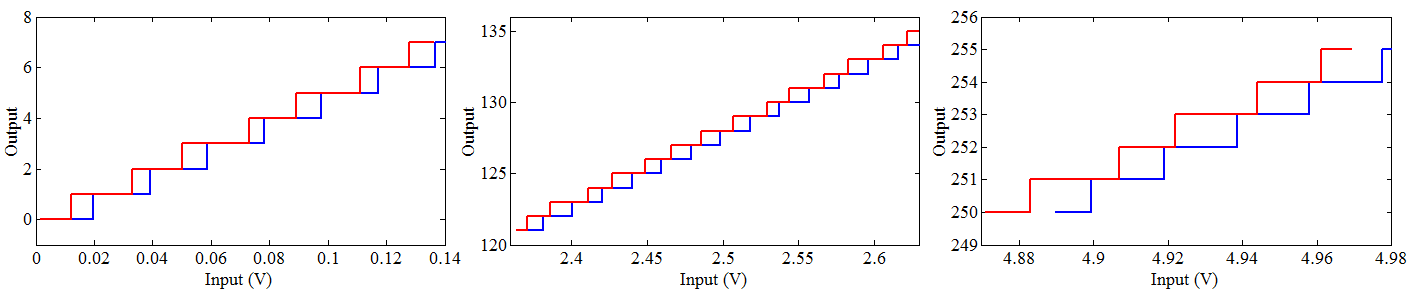
\includegraphics[width=\textwidth]{ADCresults}
    \caption{Résultats obtenus (en rouge), comparés à ${V_i = i\cdot\frac{V_{ref}}{2^8}}$ (en bleu) (${V_{ref}=4,997\mathrm{V}}$)}
    \label{fig:ADCres1}
  \end{subfigure}
  \\
  \begin{subfigure}[b]{\textwidth}
    \centering
    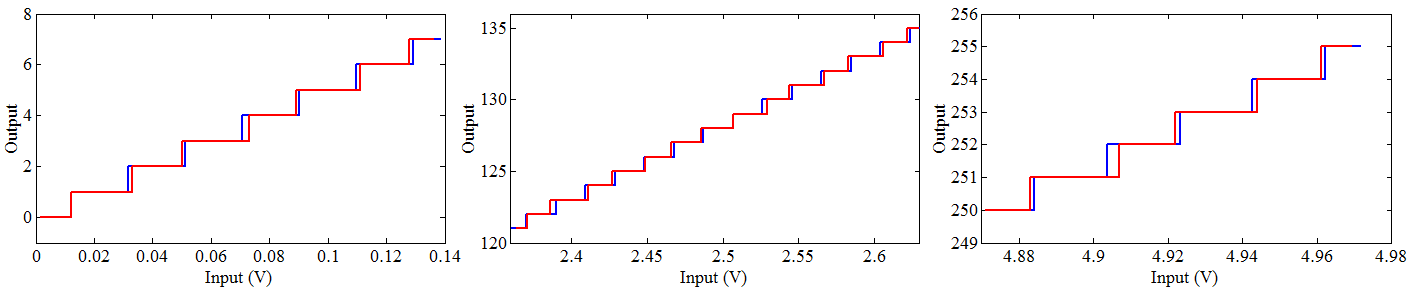
\includegraphics[width=\textwidth]{ADCresults_lincorr}
    \caption{Résultats obtenus (en rouge), comparés à ${V_i = V_{min}+i\cdot\frac{V_{max}-V_{min}}{2^n}}$ (en bleu) (${V_{min}=-0,0073\mathrm{V}}$, ${V_{max}=4,9816\mathrm{V}}$)}
    \label{fig:ADCres2}
  \end{subfigure}
  \\
  \begin{subfigure}[b]{\textwidth}
    \centering
    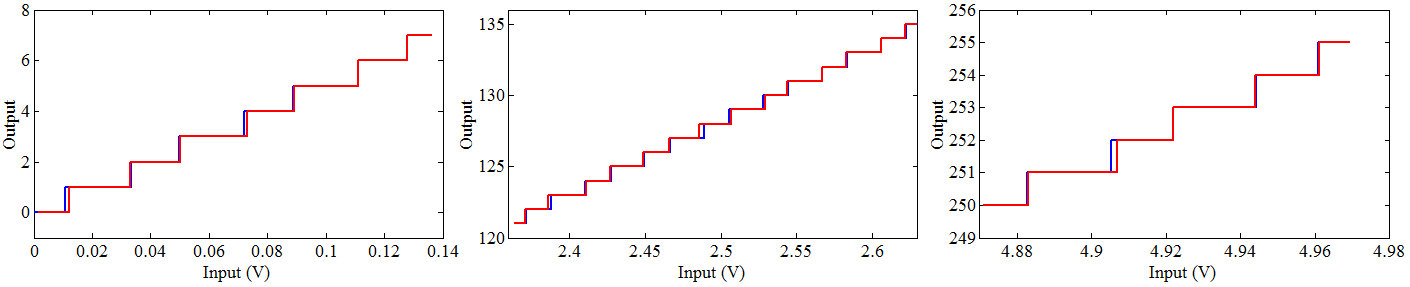
\includegraphics[width=\textwidth]{ADCresults_corr}
    \caption{Résultats obtenus (en rouge), comparés à ${V_i = V_{min}+i\cdot\frac{V_{max}-V_{min}}{2^n}}+p_i\delta V$ (en bleu) \\(${V_{min}=-0,0072\mathrm{V}}$, ${V_{max}=4,9817\mathrm{V}}$, ${\delta V=0,0015\mathrm{V}}$)}
    \label{fig:ADCres3}
  \end{subfigure}
  \caption{Résultat obtenu avec le convertisseur analogique/numérique ADC0820}
  \label{fig:ADCres}
\end{figure}

La première chose que l'on observe est un décalage permanent entre les valeurs de $V_i$ mesurées (que l'on notera $V_i^{mes}$) et les valeurs de $V_i$ théorique (que l'on notera $V_i^{th}$). On constate en effet un $offset$ moyen de $-0,0111$. On remarque toutefois que $V_i^{mes}-V_i^{th}$ augmente avec $i$ (${\langle V_i^{mes}-V_i^{th}\rangle_{i\in[1..7]}=-0,0072}$, ${\langle V_i^{mes}-V_i^{th}\rangle_{i\in[122..135]}=-0,0115}$, ${\langle V_i^{mes}-V_i^{th}\rangle_{i\in[251..255]}=-0,0150}$). 

Afin d'obtenir une meilleure approximation des résultats pratiques, on peut réutiliser la formule~:
\begin{equation*}
V_i^{th} = V_{min}+i\cdot\frac{V_{max}-V_{min}}{2^n}
\end{equation*}

On a calculé via Matlab les valeurs optimales pour $V_{min}$ et $V_{max}$ \footnote{Valeurs minimisant $\sum (V_i^{mes}-V_i^{th})^2$}, et obtenu~: ${V_{min}=-0,0073\mathrm{V}}$, ${V_{min}=4,9816\mathrm{V}}$. Les résultats correspondants sont présentés Fig.~\ref{fig:ADCres2}.

On remarque par ailleurs que pour $i$ pair $(V_i^{mes}-V_{i-1}^{mes})$ est généralement de l'ordre de $0,016\mathrm{V}$, tandis que cette valeur est généralement de l'ordre de $0,022\mathrm{V}$ pour $i$ impair. Pour représenter cette effet de la parité de $i$ sur $V_i$, on pourra utiliser la modélisation~: 
\begin{equation*}
V_i^{th} = V_{min}+i\cdot\frac{V_{max}-V_{min}}{2^n}+p_i\delta V \mathrm{~~~~avec~:~~}p_i = \begin{cases} +1 &\mathrm{si~} i\in 2\bbN \\ -1 & \mbox{sinon}\end{cases}
\end{equation*}

Là encore, on obtient avec Matlab les coefficients optimum~: ${V_{min}=-0,0072\mathrm{V}}$, ${V_{min}=4,9817\mathrm{V}}$, \\${\delta V=0,0015\mathrm{V}}$. Les résultats correspondants sont présentés Fig.~\ref{fig:ADCres3}.



Nous avons tenté de comprendre l'origine de cet effet de la parité de $i$ sur la tension de transition $V_i$. Compte tenu du principe de fonctionnement du convertisseur semi-flash, cet effet ne peut être imputé au calcul du bit de poids faible. En effet, ce dernier est donné par l'encodeur numérique encodant les quatre bits de poids faible. Il ne peut pas non plus être imputé au convertisseur numérique/analogique interne du convertisseur analogie/numérique étudié~: en effet, la sortie de ce convertisseur numérique/analogique n'est modifiée que lorsqu'un des quatre bits de poids fort est modifié. 

On en déduit que le problème est lié aux quinze ($2^-1$) comparateurs fournissant les bits en entrées de l'encodeur 4-bits des bits de poids faible. Leurs offsets seraient quasiment identiques pour les tensions de seuil $V_i$ avec $i$ pair, ainsi que pour les tensions de seuil $V_i$ avec $i$ impair.

L'hypothèse réalisée est la suivante~: tous les comparateurs utilisés ont un offset quasiment égal à $\delta V$ --- ce qui ce justifie en pratique~: cet offset est fortement lié au substrat, dont les caractéristiques peuvent être considérées comme constantes au sein du convertisseur étudié. En revanche, un convertisseur sur deux serait placé ``à l'envers''~: on code ${V < V_i}$ pour $i$ pair, et ${V > V_i}$ pour $i$ impair (ou l'inverse). Cela se justifie par une éventuelle simplification de l'encodeur 4-bits obtenue en codant un bit sur deux en entrée avec une logique négative.


\section{Le convertisseur numérique/analogique AD7524}
\label{sec:AD7524}

\subsection{Prévisions théoriques}

\exsubpart{1}

Le convertisseur numérique/analogique étudié est un CNA 8 bits à réseau R/2R : l'AD7524.

Le principe de base de la plupart des CNA à réseau R/2R repose sur l'équivalence représentée Fig.~\ref{fig:R2Rbase1}, où $V_{min}$ et $V_{max}$ sont des tensions fixées. De cette équivalence découle l'équivalence représentée Fig.~\ref{fig:R2Rbase2}, où $V_{ref}$ est une tension fixée, $B_0$, $B_1$, \dots, $B_{n-1}$ sont les bits en entrée du CNA, et~:
\begin{equation*}
V_{eq} = \left(\sum_{i=0}^{n-1}\frac{1}{2^{n-i}}B_i\right)V_{ref}
\end{equation*}

\begin{figure}[h]
  \centering
  \begin{subfigure}[b]{0.43\textwidth}
    \centering
    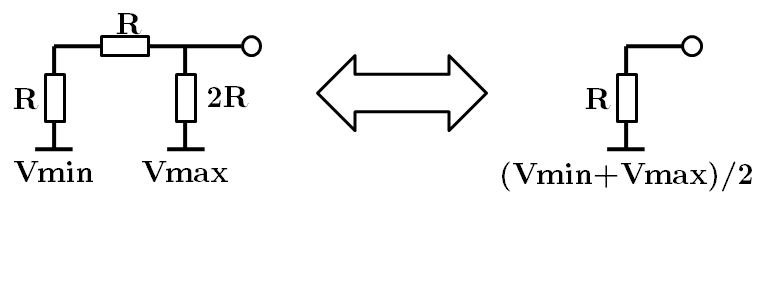
\includegraphics[width=\textwidth]{R2Rbasics}
    \caption{Équivalence de base}
    \label{fig:R2Rbase1}
  \end{subfigure}
  ~~~~
  \begin{subfigure}[b]{0.53\textwidth}
    \centering
    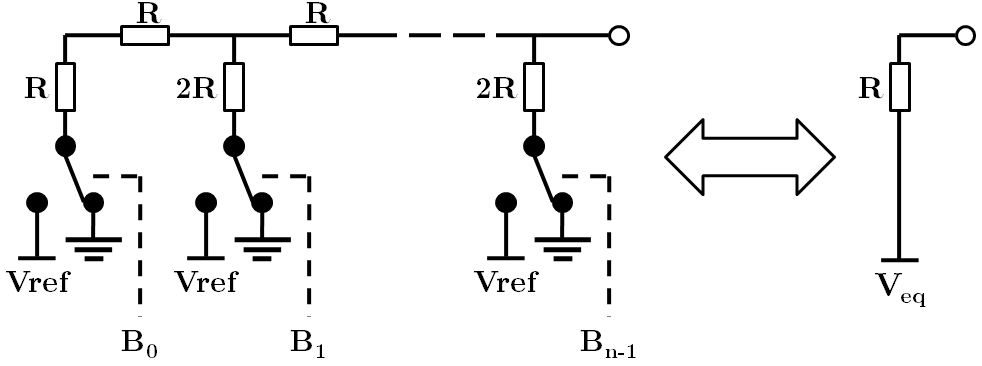
\includegraphics[width=\textwidth]{R2Rexpended}
    \caption{Équivalence en résultant}
    \label{fig:R2Rbase2}
  \end{subfigure}
  \caption{Principe de base des CNA à réseau R/2R}
\end{figure}

On utilise alors généralement un amplificateur opérationnel branché en suiveur ou en amplificateur de gain $-1$, afin d'obtenir en sortie la tension $V_eq$ indépendamment du reste du circuit.


Le fonctionnement de l'AD7524 est légèrement différent. Le circuit correspondant, tel qu'il est branché (avec notamment la sortie OUT2 branchée à la masse et l'utilisation d'un amplificateur opérationnel), est représenté Fig.~\ref{fig:AD7524} \footnote{Un condensateur, liant $V_{out1}$ et $V_{out}$, a été omis~: proposé par les datasheets, son but est d'empêcher des oscillations en sortie de l'amplificateur opérationnel. Nous nous plaçons dans le cadre d'un état déjà stabilisé, où le condensateur agit comme un interrupteur ouvert.}.

\begin{figure}[h]
  \centering
  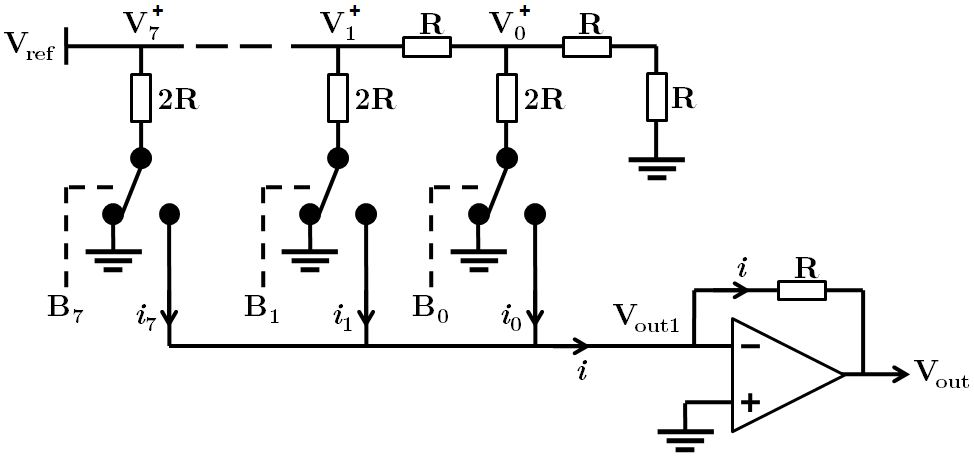
\includegraphics[width=.6\textwidth]{AD7524}
  \caption{Le convertisseur AD7524 en situation}
  \label{fig:AD7524}
\end{figure}

\begin{wrapfigure}{r}{0.3\textwidth}
  \begin{center}
    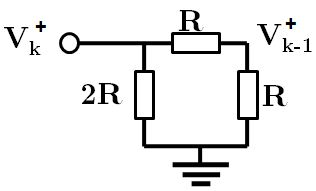
\includegraphics[width=0.2\textwidth]{AD7524eq}
  \end{center}
  \caption{Calcul des $V_k^+$}
  \label{fig:AD7524eq}
\end{wrapfigure}

L'amplificateur opérationnel fixe $V_{out1}=0$. L'équivalence présentée Fig.~\ref{fig:R2Rbase1} permet alors de calculer par récurrence les tenions $V_k^+$ (cf Fig.~\ref{fig:AD7524eq})~: $V_7^+ = V_{ref}$ et $V_{k-1}^+=\frac{V_k^+}{2}$~; d'où~: ${V_k^+=\frac{V_{ref}}{2^{7-k}}}$.

On obtient alors~:
\begin{equation*}
i = \sum_{k=0}^7 i_k = \sum_{k=0}^7 B_k \frac{V_k^+}{2R} = \frac{V_{ref}}{R} \sum_{k=0}^7 \frac{1}{2^{8-k}} B_k
\end{equation*}


Puisque $V_{out} = -R~i$, dans notre cas, on obtient ainsi pour l'ensemble des bits d'entrée $(B_0,\dots,B_7)$ un tension de sortie donnée par la formule~:
\begin{equation}
V_{out}(B_0\dots B_7) = -\left(\sum_{k=0}^{7}\frac{1}{2^{n-k}}B_k\right)V_{ref}
\label{eq:CNAeq}
\end{equation}

\exsubpart{2}

Selon la formule~\ref{eq:CNAeq}, la contribution du bit $i$ à la tension de sortie $V_{out}$ est donnée par la formule~:
\begin{equation*}
V_i^{out} = -\frac{1}{2^{8-i}}V_{ref}
\end{equation*}

Les valeurs correspondantes ont été rajoutées au tableau~\ref{tab:AD7524} des résultats théoriques.

\exsubpart{3}

Toujours selon la formule~\ref{eq:CNAeq}, on a théoriquement~:
\begin{equation*}
V_{out}(\mathtt{00000000}) = 0
\end{equation*}
et~:
\begin{eqnarray*}
V_{out}(\mathtt{11111111}) &=& -\left(\sum_{i=0}^{7}\frac{1}{2^{8-i}}B_i\right)V_{ref} = -(1-\frac{1}{2^8})V_{ref}\\
V_{out}(\mathtt{11111111}) &=& -4,9775\mathrm{V}
\end{eqnarray*}


\subsection{Mesures}

\exsubpart{1}

Cette fois encore, la tension d'alimentation utilisée pour le convertisseur, servant aussi de tension de référence $V_{ref}$, est fournie par une alimentation stabilisée~; et est précisément de~: ${V_{ref}=\mathrm{4.997 V}}$.


\exsubpart{2,3}

Expérimentalement, on mesure la contribution $V_i^{out}$ de chaque bit $i$ en mettant en entrée du CNA tous les bits à zéro, excepté le bit $i$. Ainsi, on considère~:
\begin{equation*}
V_i^{out} = V_{out}(\delta_{0,i}\delta_{1,i}\delta_{2,i}\delta_{3,i}\delta_{4,i}\delta_{5,i}\delta_{6,i}\delta_{7,i}) \mathrm{~~~~avec~:~~}\delta_{j,i} = \begin{cases} \mathtt{1} &\mathrm{si~} i=j \\ \mathtt{0} & \mbox{sinon}\end{cases}
\end{equation*}

Les résultats obtenus sont présentés dans le tableau~\ref{tab:AD7524}. $V_i^{out,th}$ désigne la valeur théorique de la contribution du bit $i$ à la tension de sortie $V_{out}$, tandis que $V_i^{out,mes}$ en désigne la valeur mesurée expérimentalement.

%TODO: Constater notamment qu'expérimentalement on a PAS : $ V_{out}(\mathtt{11111111}) = \sum_{i=0}^7 V_i^{out} $ ??   => offset sur chaque bit, une fois sur vout(11111111). Voir en faisant Vout(11111111)-offset.


\begin{table}[h]
\caption{Résultats obtenus lors de l'étude du convertisseur AD7524}
\label{tab:AD7524}
\centering
\begin{tabular}{|c|c|c|c|c|c|c|c|c|}
\hline
$i$ & 0 & 1 & 2 & 3 & 4 & 5 & 6 & 7 \\
\hline
$V_i^{out,th}$ (V) & -0,0195 & -0,039 & -0,0781 & -0,1562 & -0,3123 & -0,6246 & -1,2493 & -2,4985 \\
\hline
$V_i^{out,mes}$ (V) & -0,019 & -0,039 & -0,078 & -0,157 & -0,314 & -0,628 & -1,258 & -2,518 \\
\hline
$\sum_{j\leq i}V_j^{out,mes}$ (V) & -0,019 & -0,058 & -0,136 & -0,293 & -0,607 & -1,235 & -2,493 & -5,011 \\
\hline
\end{tabular}

\vspace{10pt}
\begin{tabular}{|c|c|c|}
\hline
Entrée & \texttt{00000000} & \texttt{11111111} \\
\hline
$V_{out}$ théorique (V) & 0 & -4,9775 \\
\hline
$V_{out}$ mesurée (V) & 0,001 & -5,04 \\
\hline
\end{tabular}
\end{table}

On remarque que l'on a notamment~: $\forall i\in [1..7], \sum_{j<i}V_j^{out,mes} < V_i^{out,mes}$.

Ainsi, le convertisseur numérique/analogique étudié est monotone. En effet, cela montre que si ${\forall j>i, B'_j=B_j}$, $B_i=0$, $B'_i=1$, ${\forall j<i, B_j=1}$ et ${\forall j<i, B'_j=0}$, alors~: \begin{equation*}V_i^{out,mes}(B_7B_6B_5B_4B_3B_2B_1B_0) < V_i^{out,mes}(B'_7B'_6B'_5B'_4B'_3B'_2B'_1B'_0)\end{equation*} \\(Par exemple~: $V_i^{out,mes}(B_7B_6B_5B_4\mathtt{0111}) < V_i^{out,mes}(B'_7B'_6B'_5B'_4\mathtt{1000})$.)

Les écarts entre les valeurs théoriques et mesurées pour $V_{out}(\mathtt{00000000})$ et $V_{out}(\mathtt{11111111})$ s'explique notamment par un mismatch entre les résistances liant les sorties OUT1 et R\_FDBK au sein du convertisseur AD7524, ainsi que par les imperfections de l'amplificateur opérationnel (offset et gain fini). De ces imperfections, il résulte un offset en sortie de l'ensemble du convertisseur, amplificateur opérationnel inclus, ainsi qu'une erreur sur le gain.

L'offset est donné par~: 
\begin{equation*}
V_{offset}=V_{out}^{mes}(\mathtt{00000000})-V_{out}^{th}(\mathtt{00000000})=0,001\mathrm{V}
\end{equation*}
et l'erreur sur le gain est donnée par~:
\begin{equation*}
\delta_G=\frac{(V_{out}^{mes}(\mathtt{11111111})-V_{out}^{mes}(\mathtt{00000000}))-(V_{out}^{th}(\mathtt{11111111})-V_{out}^{th}(\mathtt{00000000}))}{V_{out}^{th}(\mathtt{11111111})-V_{out}^{th}(\mathtt{00000000})}=1,25\mathrm{\%}
\end{equation*}

On peut alors préciser la formule fournissant $V_{out}$, en prenant~:
\begin{equation*}
V_{out}^{th}(B_0\dots B_7) = V_{offset}-(1+\delta_G)\left(\sum_{k=0}^{7}\frac{1}{2^{n-k}}B_k\right)V_{ref} = V_{offset}-\left(\sum_{k=0}^{7}\frac{1}{2^{n-k}}B_k\right)\widetilde{V_{ref}}
\end{equation*}
avec~: $\widetilde{V_{ref}} = (1+\delta_G)V_{ref} = -\frac{V_{out}^{mes}(\mathtt{11111111})-V_{out}^{mes}(\mathtt{00000000})}{1-\frac{1}{2^8}} = 5,061\mathrm{V}$



\section{Chaine de conversion A/N - N/A}


\subsection{Montage étudié}

On connecte maintenant les 8 bits de sortie du convertisseur analogique/numérique ADC0820 étudié section~\ref{sec:ADC0820} aux 8 bits d'entrée du convertisseur numérique/analogique AD7524 étudié section~\ref{sec:AD7524}.

On notera $V_{in}$ la tension imposée en entrée du montage (tension d'entrée du convertisseur analogique/numérique), et $V_{out}$ la tension obtenue en sortie (tension de sortie du convertisseur numérique/analogique). 

Dans le cadre de convertisseurs parfaits, d'une fréquence d'échantillonnage infinie et d'un nombre de bits infini, on aurait donc : $V_{out}=-V_{in}$. Dans notre cas, on obtient évidemment une approximation~; et les différences entre $V_{out}$ et $-V{in}$ seront discutées plus bas.

Pour cela, un amplificateur opérationnel permet d'obtenir en plus de la sortie du montage la tension~: ${V_{err}=-(V_{out}+V_{in})}$.

\subsection{Mesures}

\exsubpart{1}

Afin d'observer les effets de la chaîne AN-NA sur le signal (échantillonnage, quantification\dots), on applique en entrée un signal $V_{in}$ triangulaire d'amplitude $4\mathrm{V}$ et de moyenne $2,5\mathrm{V}$. On en fera varier la tension $f_{in}$.

\noindent \textbf{\underline{Quantification}}.

Afin d'observer l'effet de la quantification, sans être perturbé par l'échantillonnage, on utilise en entrée un signal lent~: $f_{in}\ll f_{ech}$ (où $f_{ech}$ désigne la fréquence d'échantillonnage des convertisseurs, que l'on sait de l'ordre de $20\mathrm{kHz}$). Typiquement, on utilisera ici $f_{in} = \mathrm{0.5 Hz}$.

Les résultats expérimentaux obtenus sont fournis Fig.~\ref{fig:slow}.

%\begin{figure}[h!]
%  \centering
%  \hfill
%  \begin{subfigure}[b]{0.4\textwidth}
%    \centering
%    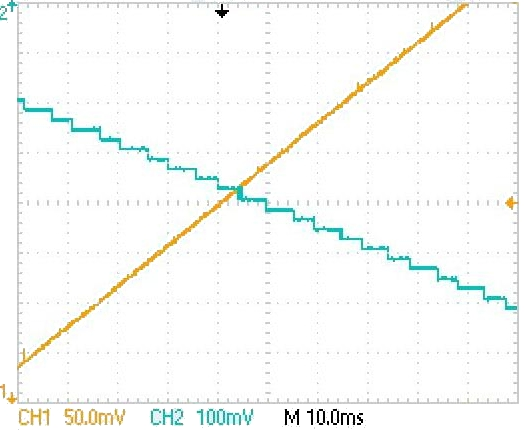
\includegraphics[width=\textwidth]{data/TEK0018_}
%    \caption{$V_{out}=f(t)$ (CH1), $V_{out}=f(t)$ (CH2)}
%    \label{fig:slowT}
%  \end{subfigure}
%  \hfill
%  \begin{subfigure}[b]{0.4\textwidth}
%    \centering
%    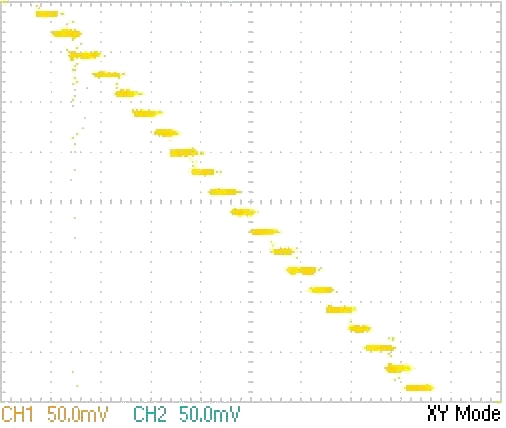
\includegraphics[width=\textwidth]{data/TEK0017_}
%    \caption{$V_{out}=f(V_{in})$}
%    \label{fig:slowXY}
%  \end{subfigure}
%  \hfill
%  \caption{$V_{in}$ et $V_{out}$ pour un signal d'entrée triangulaire d'amplitude 2V (4V crête à crête)}
%  \label{fig:slow}
%\end{figure}

Le phénomène s'observe bien lorsque l'on trace $V_{out}=f(V_{in})$ (cf. Fig.~\ref{fig:slowXY}). On y observe des ``marches'' de hauteurs et largeurs régulières, de l'ordre de $\frac{V_{ref}}{2^8}\approx\mathrm{19,5 mV}$. Ces marches sont continues sur le plan horizontal, mais pas sur le plan vertical~: à chaque valeur de $V_{out}$ correspond plusieurs valeurs de $V_{in}$. Plus simplement, sans prendre en compte d'éventuels offsets ou erreurs de gain, lors de la conversion $V_{in}\rightarrow V_{out}$, $-V_{in}$ est ``rabattu'' sur la valur possible de $V_{out}$ la plus proche.

On introduit ainsi un erreur de quantification comprise entre $-\frac{1}{2}\frac{V_{ref}}{2^8}$ et $+\frac{1}{2}\frac{V_{ref}}{2^8}$.
%TODO: sur signal 0,5HZ > Verr zoomé : dans de scie relativement régulière, d'amplitude VLSB



\noindent \textbf{\underline{Échantillonnage}}.

%\begin{figure}[h!]
%  \centering
%  \hfill
%  \begin{subfigure}[b]{0.3\textwidth}
%    \centering
%    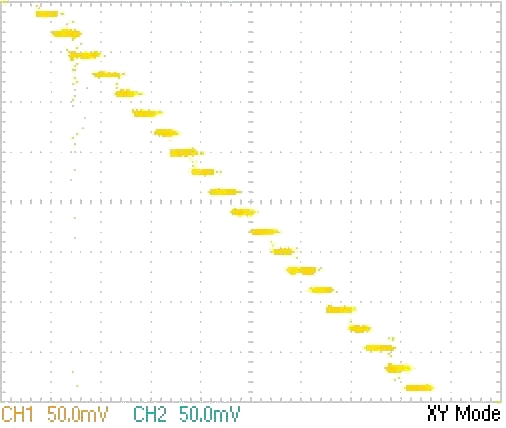
\includegraphics[width=\textwidth]{data/TEK0017_}
%    \caption{$f_{in}=$0,5 Hz)}
%    \label{fig:slowXY_}
%  \end{subfigure}
%  \hfill
%  \begin{subfigure}[b]{0.3\textwidth}
%    \centering
%    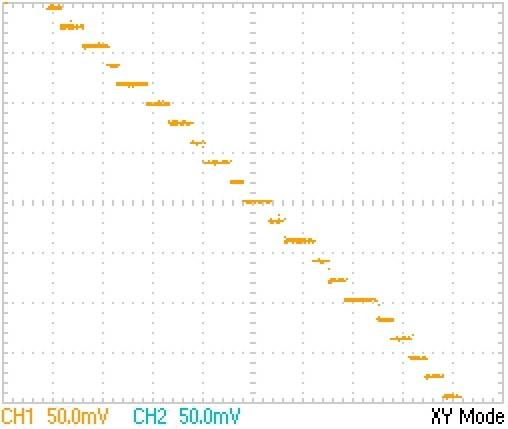
\includegraphics[width=\textwidth]{data/TEK0000_}
%    \caption{$f_{in}=$50 Hz)}
%    \label{fig:midXY}
%  \end{subfigure}
%  \hfill
%  \begin{subfigure}[b]{0.3\textwidth}
%    \centering
%    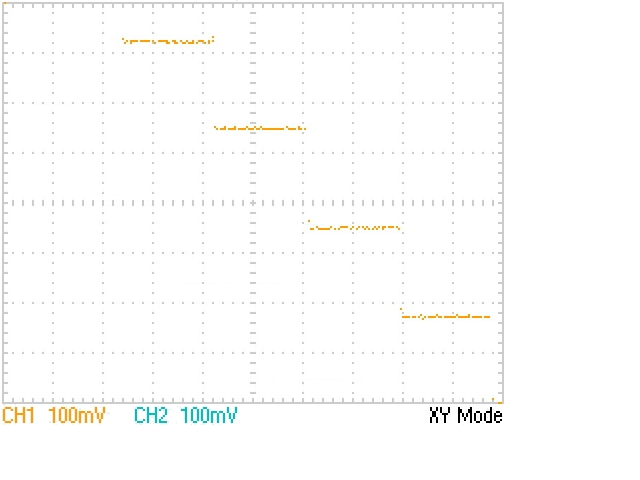
\includegraphics[width=\textwidth]{data/TEK0020_}
%    \caption{$f_{in}=$0,5 Hz)}
%    \label{fig:fastXY}
%  \end{subfigure}
%  \hfill  \caption{$V_{out}=f(V_{in})$ pour différentes fréquences d'entrées}
%  \label{fig:slow}
%\end{figure}
%
%\begin{sidewaysfigure}
%  \centering
%  \begin{subfigure}{0.28\textwidth}
%          \centering
%          \includegraphics[width=\textwidth]{pb31}
%          \caption{Basic data-flow graph}
%          \label{fig:pb31}
%  \end{subfigure}
%  ~~~
%  \begin{subfigure}{0.65\textwidth}
%    \centering
%    \begin{subfigure}{\textwidth}
%            \centering
%            \includegraphics[width=\textwidth]{pb32}
%            \caption{Reduced data-flow graph, using tree height reduction}
%            \label{fig:pb32}
%    \end{subfigure}
%    \\
%    \begin{subfigure}{0.9\textwidth}
%            \centering
%            \includegraphics[width=\textwidth]{pb33}
%            \caption{Reduced data-flow graph, using constant propagation and operator strength reduction}
%            \label{fig:pb33}
%    \end{subfigure}
%  \end{subfigure}
%  \caption{Data-flow graphs for Problem III}
%\end{sidewaysfigure}

\begin{sidewaysfigure}
	\centering
	\begin{subfigure}[b]{0.3\textwidth}
		\begin{subfigure}[b]{\textwidth}
			\centering
			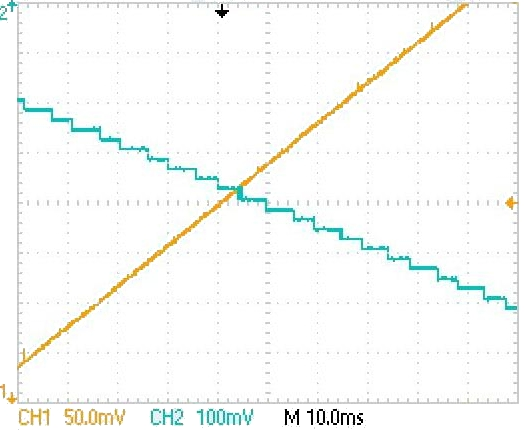
\includegraphics[width=\textwidth]{data/TEK0018_}
			\caption{\centering $f_{in}=\mathrm{0,5 Hz}$\\$V_{out}=f(t)$ (CH1), $V_{out}=f(t)$ (CH2)}
			\label{fig:slowT}
		\end{subfigure}
		\\
		\begin{subfigure}[b]{\textwidth}
			\centering
			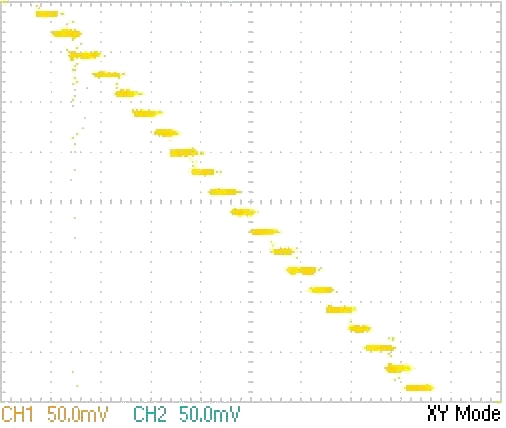
\includegraphics[width=\textwidth]{data/TEK0017_}
			\caption{\centering $f_{in}=\mathrm{0,5 Hz}$\\$V_{out}=f(V_{in})$}
			\label{fig:slowXY}
		\end{subfigure}
	\end{subfigure}
	\hfill
	\begin{subfigure}[b]{0.3\textwidth}
		\begin{subfigure}[b]{\textwidth}
			\centering
			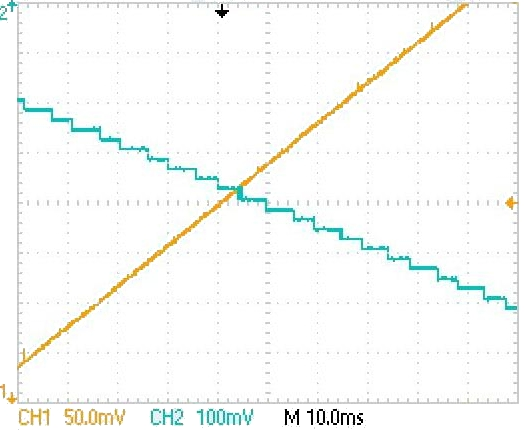
\includegraphics[width=\textwidth]{data/TEK0018_}
			\caption{\centering $f_{in}=\mathrm{0,5 Hz}$\\$V_{out}=f(t)$ (CH1), $V_{out}=f(t)$ (CH2)}
			\label{fig:midT}
		\end{subfigure}
		\\
		\begin{subfigure}[b]{\textwidth}
			\centering
			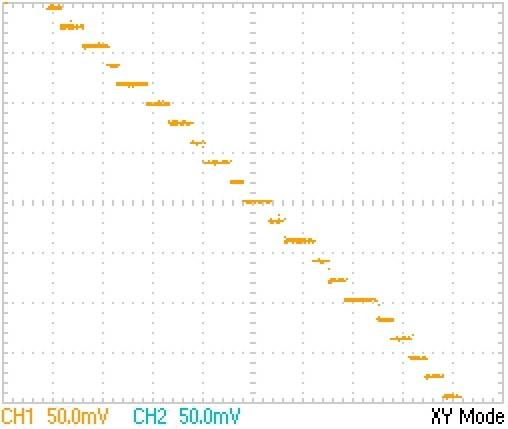
\includegraphics[width=\textwidth]{data/TEK0000_}
			\caption{\centering $f_{in}=\mathrm{0,5 Hz}$\\$V_{out}=f(V_{in})$}
			\label{fig:midXY}
		\end{subfigure}
	\end{subfigure}
	\hfill
	\begin{subfigure}[b]{0.3\textwidth}
		\begin{subfigure}[b]{\textwidth}
			\centering
			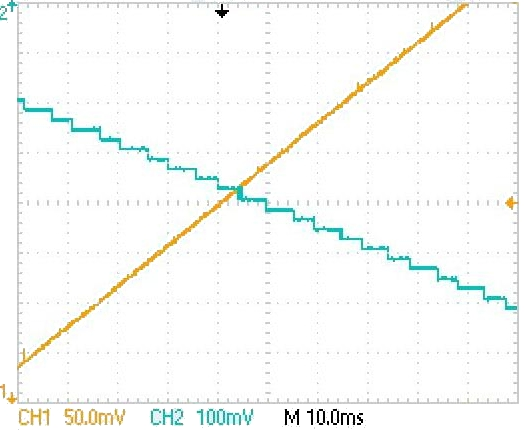
\includegraphics[width=\textwidth]{data/TEK0018_}
			\caption{\centering $f_{in}=\mathrm{0,5 Hz}$\\$V_{out}=f(t)$ (CH1), $V_{out}=f(t)$ (CH2)}
			\label{fig:fastT}
		\end{subfigure}
		\\
		\begin{subfigure}[b]{\textwidth}
			\centering
			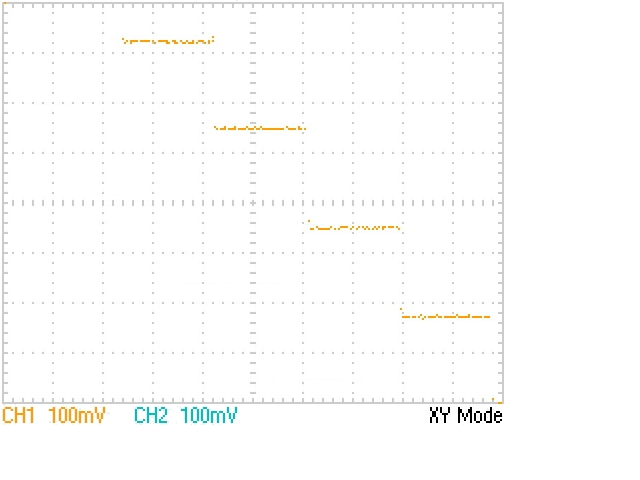
\includegraphics[width=\textwidth]{data/TEK0020_}
			\caption{\centering $f_{in}=\mathrm{0,5 Hz}$\\$V_{out}=f(V_{in})$}
			\label{fig:fastXY}
		\end{subfigure}
	\end{subfigure}	
	\caption{Data-flow graphs for Problem III}
\end{sidewaysfigure}

% Erreurs :
%  - Echantillonage
%      > Verr sur fréq rapide : largeur régulière, estimation de la fréq d'échantillonage
%      > Escalier sur fréq plus rapide : marche de longueur non régulière (dVin ou 2*dVin)
%TODO  > Escalier sur fréq beaucoup plus rapide : marche de longueur non régulière et valeurs manquantes
%  - Gain
%      > Verr dézoomé, fréq raisonnable
%  - Retard
%      > Verr dézoomé, fréq haute : au Verr précédemment affiché, on ajoute un signal carré



\end{document}